\section{Zettelumfrage}

\subsection{Beschreibung}
Hier werden einfache Papierzettel als Umfragemedium genutzt. Auf diesen stehen spezifische Fragen für einzelne Abteilungen oder Zielgruppen eines Unternehmens. Dabei können verschiedene Umfragebögen für diverse Abteilungen oder Gruppen erstellt und bei diesen explizit ausgelegt werden. Bei der Auslage der Zettel ist darauf zu achten, dass diese immer ausschließlich für die gewählte Zielgruppe erreichbar, jedoch gleichzeitig gut zugänglich sind. Die abgedruckten Fragen können direkt von der bestehenden PulseShift-Applikation entnommen werden. Durch diese Vorgehensweise ist eine Authentisierung der Mitarbeiter nicht mehr notwendig, da nur die gewünschten Zielpersonen Zugang zu den entsprechenden Zetteln haben. Fraglich ist, wie die Mitarbeiter dazu motiviert werden, solche Zettel auszufüllen. Ein weiteres Problem ergibt sich bei der Auswertung der Zettel. So müsste entweder ein spezielles Programm zur Auswertung geschrieben werden oder eine händische Auswertung erfolgen. Beide Optionen erweisen sich als kostenintensiv und sind mit einem hohen Aufwand verbunden.

\subsection{Mockups}

\begin{figure}[H]
\centering
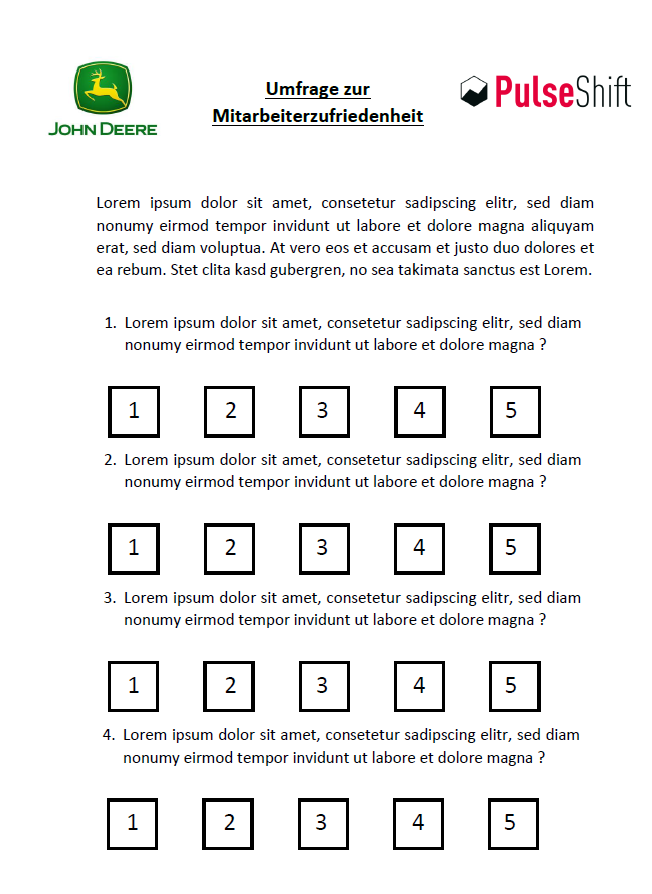
\includegraphics[width=0.9\textwidth]{images/portfolio/paper_survey}
\caption[Mockup Zettelumfrage]{Mockup Zettelumfrage}
\label{fig:portfolio:paper_survey}
\end{figure}

\subsection{Kostenfaktoren}

\begin{itemize}
\item Papier (z.B. Amazon Versando:	6 € / 500 Stück)
\item Tinte (z.B. Catridge Duck Black: 50 € / 500 Stück)
\end{itemize}

Hierbei handelt es sich nur um die Materialkosten für die gedruckten Zettel. Zusätzlich zu beachten sind die Kosten, die bei der Auswertung der Zettel anfallen. Solche sind beispielsweise Kosten zur Erstellung einer Auswertungs-Software oder Kosten für die manuelle Bearbeitung der Zettel. Diese sind aber sehr schwer zu kalkulieren und werden daher vorerst nicht geschätzt.

\subsection{Beurteilung des Projektteams}
\subsubsection{Vorteile}

\begin{itemize}
\item Keine IT-Implementierung seitens des Unternehmens benötigt
\item Schnelle und einfache Beantwortung der Zettel durch Mitarbeiter
\item Geringe Kosten und einfacher Prozess für die Erstellung der Zettel
\item Kein Authentisierungsprozess benötigt
\end{itemize}

\subsubsection{Nachteile}

\begin{itemize}
\item Aufwändiger Auswertungsprozess
\item Hohe Kosten bei der Auswertung der Zettel
\item Zielgruppen müssen lokal von anderen Gruppen trennbar sein $\rightarrow$ Wo werden die Zettel ausgelegt?
\item Zettel müssen gedruckt werden
\item Die entsprechenden Fragen müssen händisch in ein Dokument eingetragen werden
\end{itemize}

\subsubsection{Bewertung und Potential}
Für die Mitarbeiter ist die Umfrage schnell und einfach durchzuführen. Es müssen keine weiteren Applikationen installiert oder sonstige technische Voraussetzungen geschaffen werden. Allerdings erfordert die Umfrage einen hohen Arbeitsaufwand in der Vorbereitung und Auswertung. Die geringen Kosten für die Zettel selbst sind jedoch zu vernachlässigen. Insbesondere durch den Medienbruch in der Auswertung und durch den fehlenden Anreiz für die Mitarbeiter stellen die Zettel keinen geeigneten Umfragekanal dar.

\subsection{Feedback und Beurteilung durch PulseShift}

PulseShift sieht die Umsetzung einer Zettelumfrage nicht als sinnvoll an, da der Aufwand zur Auswertung der Zettel zu hoch ist. Außerdem wird der Kanal Zettelumfrage nicht als innovativ genug betrachtet, um sich von Wettbewerbern abzugrenzen.

\subsection{Weiteres Vorgehen}

Der Kanal Zettelumfrage wird sowohl vom Projektteam als auch von PulseShift kritisch betrachtet. Er wird nicht weiter verfolgt.
